\documentclass{article}

\usepackage{amsmath,amssymb}
\usepackage{tikz}
\usepackage{pgfplots}
\usepackage{xcolor}
\usepackage[left=2.1cm,right=3.1cm,bottom=3cm,footskip=0.75cm,headsep=0.5cm]{geometry}
\usepackage{enumerate}
\usepackage{enumitem}
\usepackage{marvosym}
\usepackage{tabularx}
\usepackage{multirow}

\usepackage[utf8]{inputenc}

\renewcommand*{\arraystretch}{1.4}

\newcolumntype{L}[1]{>{\raggedright\arraybackslash}p{#1}}
\newcolumntype{R}[1]{>{\raggedleft\arraybackslash}p{#1}}
\newcolumntype{C}[1]{>{\centering\let\newline\\\arraybackslash\hspace{0pt}}m{#1}}

\title{\textbf{Rechtfertigung der Staatstätigkeit, Hausaufgabe 3}}
\author{\textsc{Henry Haustein}}
\date{}

\begin{document}
	\maketitle
	
	\section*{Aufgabe 1}
	\begin{enumerate}[label=(\alph*)]
		\item Die Straße würde 20 Mio. Euro kosten, aber einen Nutzen von $2\cdot 14$ Mio. Euro bringen. Aus gesamtwirtschaftlicher Sicht lohnt es sich also die Straße zu bauen.
		\item Auszahlungsmatrix, der Zeilenspieler wird zuerst genannt:
		\begin{center}
			\begin{tabular}{C{0.5cm}c|c|c}
				& & \multicolumn{2}{c}{\textbf{Bedorf}} \\
				& & bauen & nicht bauen \\
				\hline
				\multirow{2}{0.5cm}{\rotatebox[origin=c]{90}{\textbf{Adorf}}} & bauen & (4,4) & (-6,14) \\
				\cline{3-4}
				& nicht bauen & (14,-6) & (0,0)
			\end{tabular}
		\end{center}
		\textit{nicht bauen} ist also eine dominante Strategie, das Nash-Gleichgewicht ist daher (nicht bauen, nicht bauen).
		\item Auszahlungsmatrix, der Zeilenspieler wird zuerst genannt:
		\begin{center}
			\begin{tabular}{C{0.5cm}c|c|c}
				& & \multicolumn{2}{c}{\textbf{Bedorf}} \\
				& & bauen & nicht bauen \\
				\hline
				\multirow{2}{0.5cm}{\rotatebox[origin=c]{90}{\textbf{Adorf}}} & bauen & (20,1) & (10,11) \\
				\cline{3-4}
				& nicht bauen & (30,-9) & (0,0)
			\end{tabular}
		\end{center}
		Falls Bedorf baut, baut Adorf nicht und falls Bedorf nicht baut, baut Adorf. \\
		Falls Adorf baut, baut Bedorf nicht und falls Adorf nicht baut, baut Bedorf nicht. \\
		Für Bedorf ist \textit{nicht bauen} eine dominante Strategie; das Nash-Gleichgewicht ist (bauen, nicht bauen)
	\end{enumerate}

	\section*{Aufgabe 2}
	\begin{enumerate}[label=(\alph*)]
		\item Die Konsumenten maximieren ihren Nutzen und der Nebenbedingung $x_i=w_i-g_i$. Es gilt weiterhin $g_i=\frac{G}{n}$ und damit $x_i=w_i-\frac{G}{n}$:
		\begin{align}
			U_i &= x_i\cdot\sqrt{G} \notag \\
			&= \left(w_i-\frac{G}{n}\right)\cdot\sqrt{G} \notag
		\end{align}
		Damit gilt
		\begin{align}
			\frac{\partial U_i}{G} &= \frac{n\cdot w_i-3G}{2n\sqrt{G}} = 0 \notag \\
			n\cdot w_i - 3G &= 0 \notag \\
			G^{opt} &= \frac{n\cdot w_i}{3} \notag
		\end{align}
		\item Der Nutzen $U_i=x_i\cdot\sqrt{G}=(w_i-g_i)\sqrt{g_i+G_{-i}}$ wird maximiert
		\begin{align}
			\frac{\partial U_i}{\partial g_i} &= -\frac{3g_i - w + 2G_{-i}}{2\sqrt{g_i+G_{-i}}} =0 \notag \\
			0 &= 3g_i - w + 2G_{-i} \notag \\
			g_i &= \frac{w-2G_{-i}}{3} \notag
		\end{align}
		Im symmetrischen Gleichgewicht gilt $G_{-i}=(n-1)g_i$, also
		\begin{align}
			g_i &= \frac{w-2(n-1)g_i}{3} \notag \\
			3g_i &= w-2ng_i + 2g_i \notag \\
			2ng_i - 2g_i + 3g_i &= w \notag \\
			(2n+1)g_i &= w \notag \\
			g_i &= \frac{w}{2n+1} \notag
		\end{align}
		\item $G^{priv} = n\cdot g_i = \frac{n\cdot w_i}{2n+1}$. Ab $n>1$ gilt $G^{priv}<G^{opt}$.
		\item Es gilt
		\begin{align}
			\frac{\partial g_i}{\partial n} &= -\frac{2w}{(2n+1)^2} < 0 \notag \\
			\frac{\partial G^{priv}}{\partial n} &= \frac{w}{(2n+1)^2} > 0 \notag
		\end{align}
		\item Für den Nutzen gilt
		\begin{align}
			U_i &= x_i\cdot\sqrt{G+T} \notag \\
			&= (w_i-g_i-t_i)\sqrt{G_{-i}+g_i + T_{-1} + t_i} \to\max \notag
		\end{align}
		Die Bedingung erster Ordnung lautet
		\begin{align}
			\frac{\partial U_i}{\partial g_i} &= \frac{3g_i + 2T_{-i} - w_i + 3t_i + 2G_{-i}}{2\sqrt{G_{-i}+g_i+T_{-i}+t_i}} = 0 \notag \\
			0 &= 3g_i + 2(n-1)t_i - w_i + 3t_i + 2(n-1)g_i \notag \\
			0 &= (2n+1)g_i + (2n+1)t_i - w_i \notag \\
			g_i &= \frac{w_i-(2n+1)t_i}{2n+1} \notag
		\end{align}
		\item Es gilt
		\begin{align}
			\frac{\partial g_i}{\partial t_i} = -1 \notag
		\end{align}
		Für jeden Euro, den der Staat zur Bereitstellung des öffentlichen Gutes ausgibt, gibt jedes Individuum einen Euro weniger aus.
	\end{enumerate}
	
	\section*{Aufgabe 3}
	\begin{enumerate}[label=(\alph*)]
		\item Die Grenzkosten betragen 30. Unter Wohlfahrtsgesichtspunkten liefert $\sum GZB = GK$ die optimale Lösung, also
		\begin{align}
			\sum GZB &= GK \notag \\
			(40-2G) + (20-G) &= 30 \notag \\
			60-3G &= 30 \notag \\
			G_{opt} &= 10 \notag
		\end{align}
		\item Für Haushalt 1 gilt:
		\begin{align}
			GZB_1 &= \alpha \cdot GK \notag \\
			40-2G &= \frac{1}{2} \cdot 30 \notag \\
			G_1 &= 12.5 \notag
		\end{align}
		Für Haushalt 2 gilt:
		\begin{align}
			GZB_2 &= (1-\alpha) \cdot GK \notag \\
			20-G &= \left(1-\frac{1}{2}\right) \cdot 30 \notag \\
			G_2 &= 5 \notag
		\end{align}
		Die Haushalte fragen verschiedene Mengen nach, aber es kann nur eine Menge bereitgestellt werden.
		\begin{center}
			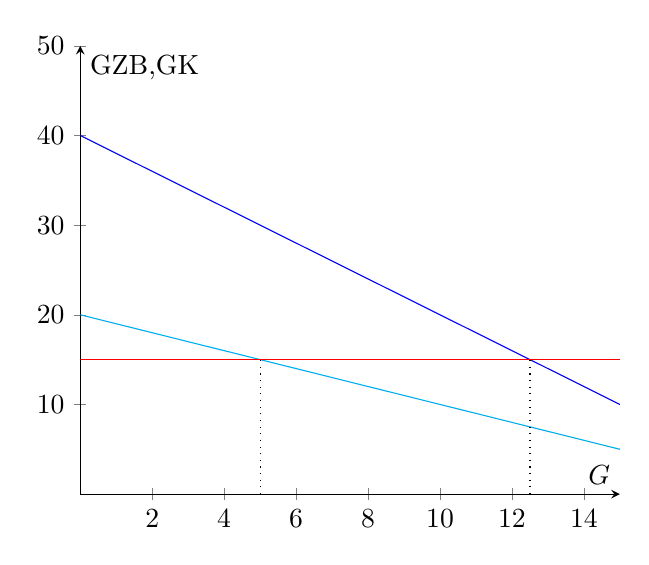
\begin{tikzpicture}
				\begin{axis}[
					xmin=0, xmax=15, xlabel=$G$,
					ymin=0, ymax=50, ylabel={GZB,GK},
					samples=400,
					axis x line=middle,
					axis y line=middle,
					domain=0:15
					]
					\addplot[mark=none,smooth,blue] {40-2*x};
					\addplot[mark=none,smooth,cyan] {20-x};
					
					\addplot[mark=none,smooth,red] {15};
					
					\draw[dotted] (axis cs: 5,0) -- (axis cs: 5,15);
					\draw[dotted] (axis cs: 12.5,0) -- (axis cs: 12.5,15);
					
				\end{axis}
			\end{tikzpicture} \\
			\textcolor{red}{$\alpha GK = (1-\alpha)GK$}, \textcolor{blue}{$GZB_1$}, \textcolor{cyan}{$GZB_2$}
		\end{center}
		\item Wir müssen $\alpha^\ast$ so wählen, dass
		\begin{align}
			GZB_1(G_{opt}) &= \alpha^\ast \cdot GK \notag \\
			40-2\cdot 10 &= \alpha^\ast \cdot 30 \notag \\
			20 &= \alpha^\ast \cdot 30 \notag \\
			\alpha^\ast &= \frac{2}{3} \notag
		\end{align}
		Der andere Haushalt muss dann $1-\alpha$ der Grenzkosten tragen, für ihn sind das $\frac{1}{3}$ der Grenzkosten.
		\begin{center}
			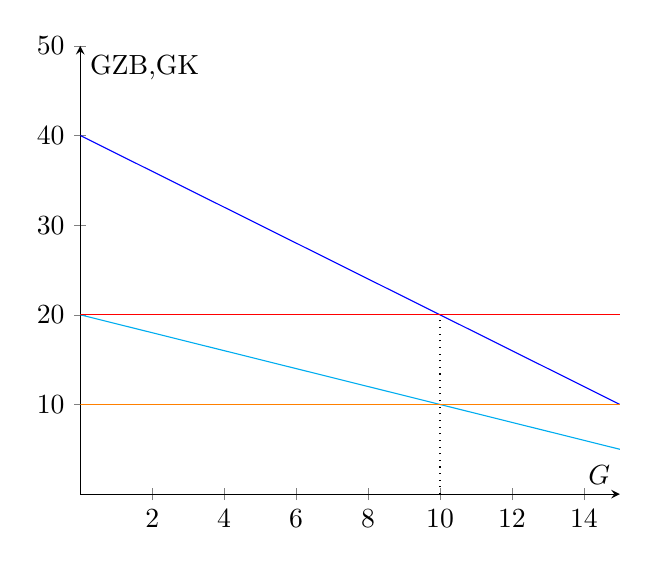
\begin{tikzpicture}
				\begin{axis}[
					xmin=0, xmax=15, xlabel=$G$,
					ymin=0, ymax=50, ylabel={GZB,GK},
					samples=400,
					axis x line=middle,
					axis y line=middle,
					domain=0:15
					]
					\addplot[mark=none,smooth,blue] {40-2*x};
					\addplot[mark=none,smooth,cyan] {20-x};
					
					\addplot[mark=none,smooth,red] {20};
					\addplot[mark=none,smooth,orange] {10};
					
					\draw[dotted] (axis cs: 10,0) -- (axis cs: 10,20);
					
				\end{axis}
			\end{tikzpicture} \\
			\textcolor{blue}{$GZB_1$}, \textcolor{cyan}{$GZB_2$}, \textcolor{red}{$\alpha\cdot GK$}, \textcolor{orange}{$(1-\alpha)\cdot GK$}
		\end{center}
	\end{enumerate}

	\section*{Aufgabe 4}
	\begin{enumerate}[label=(\alph*)]
		\item Für den Haushalt A ist die Lagrange-Funktion
		\begin{align}
			L = x_A\cdot G^2 - \lambda(12-x_A - \alpha G) \notag
		\end{align}
		Die Bedingungen erster Ordnung lauten
		\begin{align}
			\frac{\partial L}{\partial x_A} &= G^2 + \lambda =0 \notag \\
			\lambda &= -G^2 \notag \\
			\frac{\partial L}{\partial G} &= 2Gx_A + \alpha\lambda = 0 \notag \\
			0 &= 2Gx_A - \alpha G^2 \notag \\
			0 &= 2x_A - \alpha G \notag \\
			G &= 2\frac{x_A}{\alpha} \notag
		\end{align}
		Einsetzen in die Budgetrestriktion ergibt
		\begin{align}
			12 &= x_A + \alpha G  \notag \\
			&= x_A + 2x_A \notag \\
			x_A &= 4 \notag
		\end{align}
		und damit $G=\frac{8}{\alpha}$. Für den Haushalt B gilt
		\begin{align}
			L = x_B^2\cdot G - \lambda(16-x_B-(1-\alpha)G) \notag
		\end{align}
		Die Bedingungen erster Ordnung lauten
		\begin{align}
			\frac{\partial L}{\partial G} &= x_B^2 + (1-\alpha)\lambda = 0 \notag \\
			\lambda &= -\frac{x_B^2}{1-\alpha} \notag \\
			\frac{\partial L}{\partial x_B} &= 2x_B\cdot G + \lambda = 0 \notag \\
			0 &= 2x_B\cdot G - \frac{x_B^2}{1-\alpha} \notag \\
			2G &= \frac{x_B}{1-\alpha} \notag \\
			G &= \frac{x_B}{2(1-\alpha)} \notag
		\end{align}
		Einsetzen in die Budgetrestriktion ergibt
		\begin{align}
			16 &= x_B + (1-\alpha)G \notag \\
			&= x_B + \frac{x_B}{2} \notag \\
			x_B &= \frac{32}{3} \notag
		\end{align}
		und damit $G=\frac{16}{3(1-\alpha)}$.
		\item Die $G$'s müssen gleich sein, also
		\begin{align}
			\frac{8}{\alpha} &= \frac{16}{3(1-\alpha)} \notag \\
			\alpha &= \frac{3}{5} \notag
		\end{align}
		und damit $G=\frac{40}{3}$.
	\end{enumerate}

	\section*{Aufgabe 5}
	\begin{enumerate}[label=(\alph*)]
		\item Alternative A hat eine Zahlungsbereitschaft von 175, Alternative B von 195 und Alternative C von 100. Damit sollte B angeschafft werden.
		\item Es gilt
		\begin{center}
			\begin{tabular}{c|ccc|c}
				& Alternative A & Alternative B & Alternative C & Steuer \\
				\hline
				$\sum$ ZB ohne Konsument 1 & 75 & \textbf{145} & 100 & 0 \\
				$\sum$ ZB ohne Konsument 2 & \textbf{175} & 125 & 50 & 50 \\
				$\sum$ ZB ohne Konsument 3 & 150 & \textbf{195} & 50 & 0 \\
				$\sum$ ZB ohne Konsument 4 & \textbf{125} & 120 & 100 & 5
			\end{tabular}
		\end{center}
	\end{enumerate}

\end{document}